\chapter{Cahier des charges}\label{ch:cahier}

L'année dernière, la société constatait sur ses solutions une véritable disparité de méthodologies d'intégration pour les documents. Chaque fonctionnalité intégrait les documents de manière différente, ce qui les amenait à constater qu'il était alors compliqué de répondre rapidement à ce type de besoins.

De plus, elle avait d'une part des demandes d'importation de nouveaux fournisseurs de carburant, mais également d'autre part la création du poste de CSM (Customer Success Manager). En outre, suite à un besoin exprimé par l'un de ses grands clients, il y avait de plus en plus de besoins pour intégrer rapidement et efficacement de nouvelles typologies de documents.

Basé sur ce constat, l'entreprise a donc décidé qu'il était nécessaire de construire un outil permettant de répondre à ces besoins : le Pipeline documentaire.

Son projet était qu'à terme, cet outil leur permettrait de généraliser l'intégration des fichiers dans leur solution. Il serait donc le point d'entrée central pour tous les documents entrant dans chacun de leurs logiciels. L'ajout d'une nouvelle typologie de document serait simple et se ferait, pour la partie intégration du moins, principalement à travers le paramétrage.

La section suivante montre comment le propriétaire du produit a exprimé les besoins concernant le Pipeline documentaire.

\section{Expression des besoins}

\subsection{Concepts généraux}

Dans sa conception, ce nouvel outil devra être le plus détaché possible du reste de l'ensemble applicatif, afin d'être ensuite mis à disposition et utilisé par l'ensemble de nos logiciels, de manière simple et intégrée. Dans cette optique, l'outil devra donc être conçu pour être notre première \foreignquote{french}{Machine}, concept abordé lors de notre étude de la refonte globale, qui est donc un outil logiciel mis à disposition de l'ensemble des autres applications, mais qui reste complètement autonome.

\subsection{Composition de l'outil}

\subsubsection{Déclencheurs}

Le concept de déclencheur devra faire partie intégrante de la conception de l'outil, en suivant toujours les mêmes règles et en permettant de déclencher une intégration. Lorsqu'un déclencheur est \foreignquote{french}{appelé}, il lancera l'intégration complète. Celui-ci fournira au guide toutes les informations nécessaires ainsi que le ou les fichiers à intégrer. Cependant, chaque déclencheur sera indépendant et répondra à une intégration spécifique. Un certain nombre de déclencheurs ont été identifiés dans le schéma architectural (Figure~\ref{fig:architectural-schema}). Cependant, cette liste n'est pas exhaustive.

\subsubsection{Guide}

Dans notre outil, le guide sera le point central de l'intégration. Son rôle consistera à charger la configuration adéquate afin de réaliser l'intégration, puis à faire passer le ou les fichiers à travers la chaîne d'intégration, en fonction de la configuration préalablement mise en œuvre. En fin de compte, le guide aura pour objectif de piloter l'intégration complète du fichier, c'est-à-dire de s'assurer de son bon parcours à travers la chaîne d'intégration.


\subsubsection{Configurations}

Les fichiers de configuration devront être créés pour déclarer tout nouvel import. Chaque fichier de configuration aura un format informatique, mais restera lisible par un développeur (json, yml, etc.). Ces fichiers de configuration permettront, pour chaque type d'import, de définir ses spécificités et ainsi de déterminer chaque étape de l'import. Les principales informations incluses dans ces fichiers seront les suivantes :

\begin{itemize}
    \item Le mappage des données
    \item Les détails du fichier (encodage, extension, etc.)
    \item Le type (csv, xml, pdf, etc.)
    \item Les détails de la chaîne d'intégration (classes à utiliser, OCR à effectuer, etc.)
    \item Les traitements spécifiques à appliquer au fichier (classe de lecture spécifique, classe de mappage spécifique, etc.)
    \item \dots
\end{itemize}

\subsubsection{Chaine d'intégration}

Le guide aura pour but de déterminer, en se basant sur les informations du déclencheur et sur la configuration chargée, l'ensemble des maillons constituant la chaîne d'intégration. Celle-ci sera composée d'étapes distinctes et autonomes, permettant d'aboutir à l'intégration complète du fichier. Le guide s'assurera que le ou les fichiers passent bien à travers chaque maillon de la chaîne d'intégration.

\subsubsection{Actions transverses}

Les actions transverses devront être automatisées et aucune configuration ni code ne devra être intégré dans les parties spécifiques d'une importation. Cela signifie que le Pipeline documentaire en lui-même devra les gérer par défaut, sans intervention du développeur qui ajoute une nouvelle chaîne, un nouveau déclencheur ou une nouvelle configuration.

Les actions transverses seront les suivantes :

\begin{itemize}
    \item \textbf{Documentation automatique :} les configurations seront automatiquement analysées et généreront une documentation exploitable par un opérateur externe à la R\&D, tel que le support ou le commerce.
    \item \textbf{Tableau de bord :} un ensemble de tableaux devra rendre compte du bon fonctionnement du pipeline en temps réel, ainsi qu'un récapitulatif des intégrations récentes.
    \item \textbf{Sauvegardes sérialisées :} l'ensemble des étapes devra être sauvegardé et sérialisé à des fins d'analyse. Cet historique pourra être périodiquement purgé. Cependant, il est intéressant de conserver le fichier d'entrée et sa configuration attachée plus longtemps que la sérialisation des étapes.
\end{itemize}

\begin{figure}[ht]
    \centering
    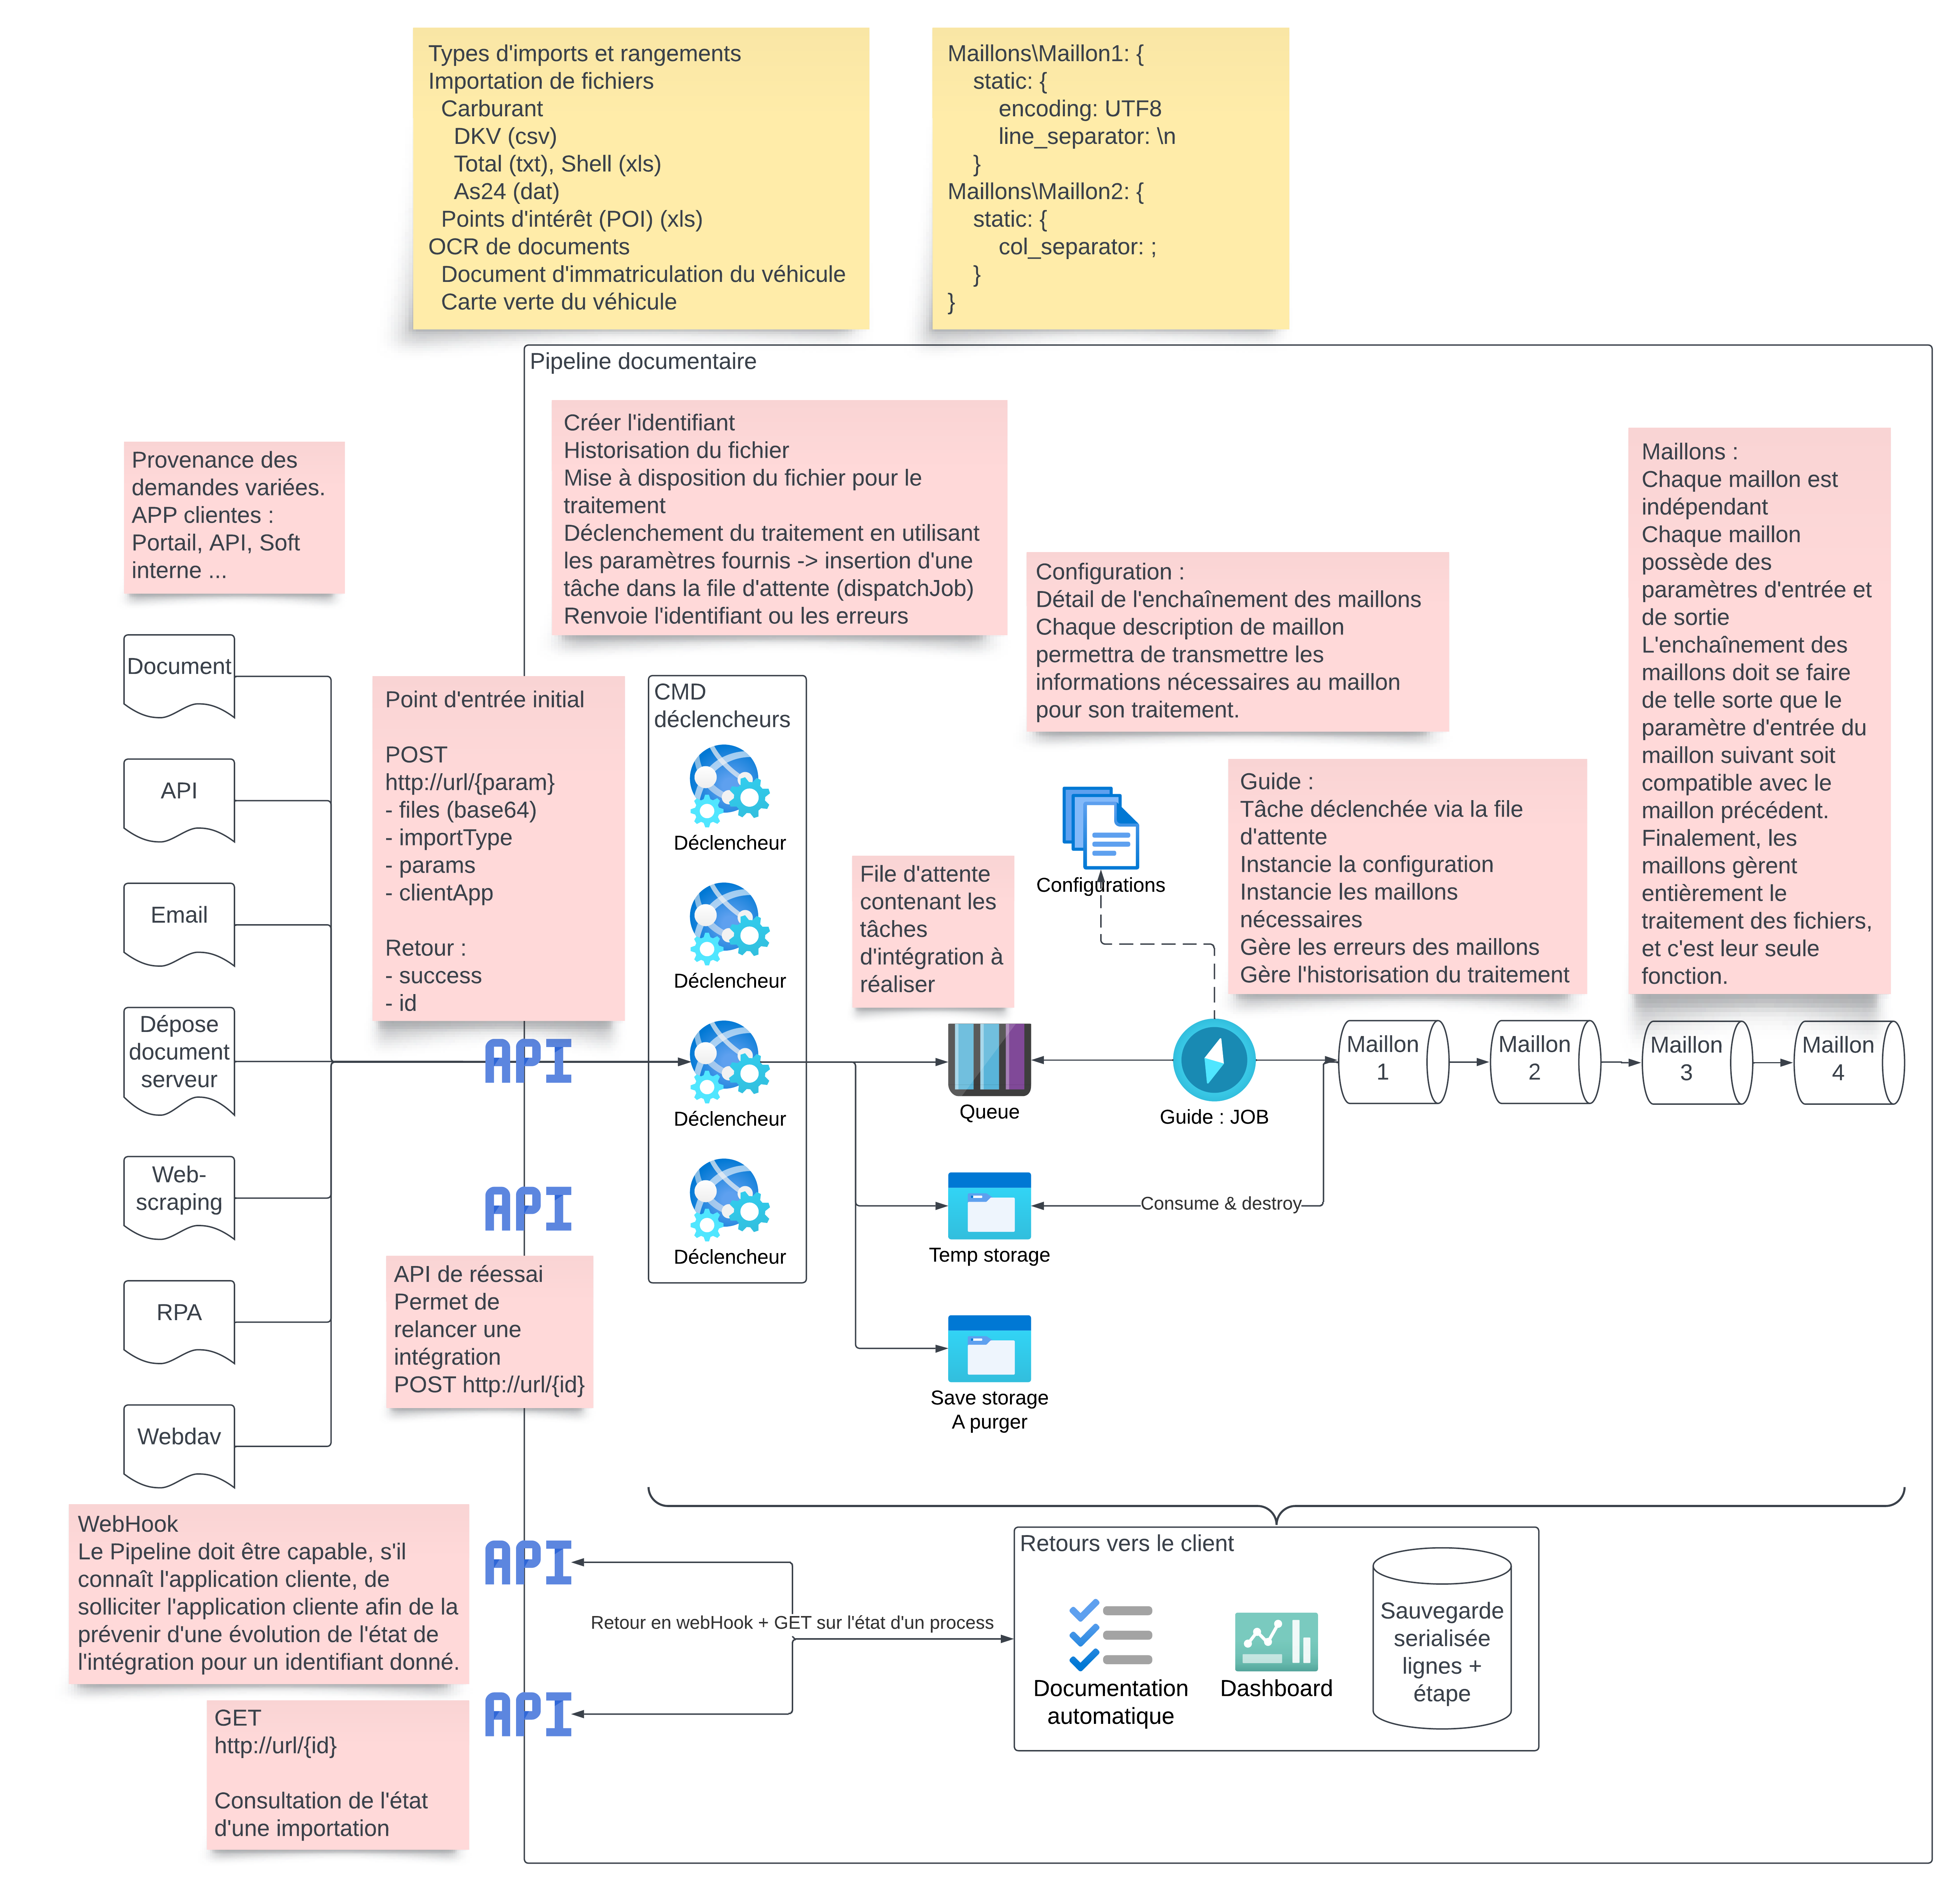
\includegraphics[width=\textwidth]{img/schema-architectural}
    \caption{Schéma architectural de Pipeline documentaire.}
    \label{fig:architectural-schema}
\end{figure}